\documentclass[14pt,compress,t,noamsthm,notheorem,table,handout]{ctexbeamer}
\usetheme{Boadilla}
\useinnertheme{circles}
\useoutertheme{shadow}
\usecolortheme{seahorse}
\usefonttheme[onlymath]{serif}
\setbeamertemplate{navigation symbols}{}
% \setbeamercovered{transparent}
\usepackage{natbib}
\usepackage{amsthm}
\usepackage{makecell}
\usepackage{multirow}
\renewcommand{\qedsymbol}{$\blacksquare$}
\bibliographystyle{unsrtnat}
\usepackage{color}
\setbeamercolor{myfootline}{bg=white,fg=blue}
\definecolor{myfoot}{rgb}{0.5,0.2,0.5}
\definecolor{darkblue}{rgb}{0.1,0,0.85}
\setbeamertemplate{headline}
  { \leavevmode\begin{beamercolorbox}[wd=\paperwidth,ht=1.25ex,dp=1ex,left]{}
    \end{beamercolorbox}}
\setbeamertemplate{footline}% 自定义页脚
  { \leavevmode\mbox{%
    \begin{beamercolorbox}[wd=.75\paperwidth,ht=2.25ex,dp=1ex,left]{myfootline}%
        \rule{2em}{0pt}\color{myfoot}\ttfamily\scriptsize%
        %\insertshortauthor~(\insertshortinstitute)
    \end{beamercolorbox}%
    \begin{beamercolorbox}[wd=.25\paperwidth,ht=2.25ex,dp=1ex,right]{myfootline}%
       {\color{myfoot}\ttfamily\scriptsize\insertframenumber{}/%
        \inserttotalframenumber\hspace*{3ex}}
    \end{beamercolorbox}}
    \vskip0pt }

\setbeamercolor{frametitle}{fg=blue,bg=white}
\setbeamertemplate{frametitle}{%
  \leavevmode\linespread{1}\large\textbf{\insertframetitle}\par
  \color{structure.fg!30!bg}\rule[6pt]{\linewidth}{2pt}\par\vspace{-1.0em}}

% \setbeamertemplate{blocks}[default] % beamer块(含定理类环境)不要阴影
\setbeamertemplate{bibliography entry title}{}{}
\setbeamertemplate{bibliography entry location}{}{}
\setbeamertemplate*{bibliography entry note}{}{}
\setbeamersize{text margin left=0.75cm, text margin right=0.75cm}

\setbeamercolor{bluebox}{fg=black,bg=blue!10}
\setbeamercolor{redbox}{fg=black,bg=red!10}
\newenvironment{Boxblue}[1][\textwidth]
  {\begin{beamercolorbox}[sep=0.1em,shadow=true,wd=#1,rounded=true,center]{bluebox}}
  {\end{beamercolorbox}}
\newenvironment{Boxred}[1][\textwidth]
  {\begin{beamercolorbox}[sep=0.1em,shadow=true,wd=#1,rounded=true,center]{redbox}}
  {\end{beamercolorbox}}
\usepackage{stmaryrd}
\usepackage{amsmath,amssymb,amsfonts,bm}
\usepackage{graphicx,xcolor}
\graphicspath{{figures/}}
\usepackage{hyperref}
\hypersetup{pdfborder=001,colorlinks=true,linkcolor=darkblue,urlcolor=blue}
\usepackage{bbding}
\newcommand{\Bullet}{{\fontsize{6pt}{6pt}\selectfont\CircleSolid}}
\newcommand{\Hand}{{\fontsize{8pt}{6pt}\selectfont\HandRight}}
\newcommand{\zhu}{{\color{blue!40}\Bullet}}
\newcommand{\zhuu}{{\color{red!80}\Hand}}
\newcommand{\labeli}{\zhu}
\newenvironment{blist}%
    {\begin{list}{{\hfill\raisebox{1.12pt}{\color{blue!60}\zhu}}}{%
     \leftmargin2em\labelwidth1.5em\labelsep0.5em
     \itemsep1ex\itemindent0pt\parsep0pt\topsep0pt}}
    {\end{list}}
\newenvironment{myitem}
  {\begin{list}{{\hfill\raisebox{0pt}{\labeli}}}{%
    \setlength{\leftmargin}{1.2em}\labelwidth0.8em\labelsep.4em%
    \itemsep1ex\parsep2pt\itemindent0pt\topsep0pt}}{\end{list}}
\newenvironment{subitem}
  {\begin{list}{{\hfill\raisebox{0pt}{-}}}{%
    \setlength{\leftmargin}{1.2em}\labelwidth0.8em\labelsep.4em%
    \itemsep0ex\parsep2pt\itemindent0pt\topsep0pt}}{\end{list}}
\usepackage{colortbl}
\usepackage{tikz}
\usetikzlibrary{arrows}
\usepackage{stmaryrd}
\usepackage{amsfonts}
\usepackage[ruled,linesnumbered]{algorithm2e}
\usepackage{float} 
\usepackage{booktabs}
\usepackage[framemethod=tikz]{mdframed}
\newmdenv[linecolor=green,middlelinewidth=1pt,%
          roundcorner=3pt,backgroundcolor=white,%
          innertopmargin=0.8em,innerbottommargin=0.5em,%
          innerleftmargin=3pt,innerrightmargin=3pt,%
          skipbelow=0.5em,skipabove=1em,%
          splittopskip=\topskip]{Block}
\newmdenv[linecolor=green,middlelinewidth=1pt,%
          roundcorner=3pt,backgroundcolor=red!5!white,%
          innertopmargin=0.5em,innerbottommargin=0.5em,%
          innerleftmargin=3pt,innerrightmargin=3pt,%
          skipbelow=0.5em,skipabove=1em,%
          splittopskip=\topskip]{redbox}
\newmdenv[linecolor=green,middlelinewidth=0.5pt,%
          %outerlinewidth=0.5pt,skipabove=0pt,
          roundcorner=3pt,backgroundcolor=white,%
          innerbottommargin=3pt,innerrightmargin=5pt,%
          innerleftmargin=5pt,leftmargin=0ex]{mathbox}
\newmdenv[linecolor=blue!5!green,middlelinewidth=0.5pt,%
          roundcorner=3pt,backgroundcolor=yellow!5,%
          % frametitle={Hello},frametitlebackgroundcolor=green!50,%
          % skipabove=2pt,skipbelow=2pt,%
          innerleftmargin=3pt,leftmargin=0ex]{notebox}
\newmdenv[linecolor=white,font={\scriptsize},%
          fontcolor=blue!85,backgroundcolor=yellow!5,%
          skipabove=1ex,skipbelow=0pt,innerbottommargin=0.5ex,%
          innerleftmargin=3pt,leftmargin=1em]{myref}

%%%%%%%%%%%%%%%%%%%%%%%%%%%%%%%%%%%%%%%%%%%%%%%%%%%%%%%%%%%%%%%%%%%%%%%%%%%%%%
\renewcommand{\thefootnote}{}% 不要编号
\setbeamertemplate{footnote}{% 首行不缩进
  \noindent\insertfootnotemark%
  \scriptsize\color{blue!85!green!85}\insertfootnotetext\par\kern1ex}
\renewcommand\footnoterule%    更改横线属性:长度,粗细,颜色
  {\color{red}\kern-3pt\rule{0.4\linewidth}{0.5pt}\par\kern2.6pt}
%%%%%%%%%%%%%%%%%%%%%%%%%%%%%%%%%%%%%%%%%%%%%%%%%%%%%%%%%%%%%%%%%%%%%%%%%%%%%%

\usepackage[many]{tcolorbox}
\tcbset{highlight math %
  style={enhanced, colframe=blue!40,colback=yellow!20,arc=4pt,boxrule=1pt}}
\newtcbox{\subsubtit}[1][]{%
  after skip=1em,boxrule=0.5pt,
  fontupper=\color{blue}\bfseries,top=0.5ex,bottom=0.5ex,
  left=1ex,right=1ex,
  colframe=green,colback=red!5!white,#1}

%\renewcommand{\baselinestretch}{1.1}
\linespread{1.1}
\setlength{\parskip}{1ex}

\usepackage{listings} %插入代码
\usepackage{xcolor}
\lstset{numbers=left, %设置行号位置
        numberstyle=\tiny, %设置行号大小
        keywordstyle=\color{blue}, %设置关键字颜色
        commentstyle=\color[cmyk]{1,0,1,0}, %设置注释颜色
        frame=single, %设置边框格式
        escapeinside=``, %逃逸字符(1左面的键),用于显示中文
        %breaklines, %自动折行
        extendedchars=false, %解决代码跨页时,章节标题,页眉等汉字不显示的问题
        xleftmargin=2em,xrightmargin=2em, aboveskip=1em, %设置边距
        tabsize=4, %设置tab空格数
        showspaces=false, %不显示空格
        basicstyle=\ttfamily,
       }
\begin{document}

%%%%% =======================================================================
\title{R语言-1}
\author{郑泽靖 \and zzjstat2023@163.com }
\institute{\normalsize 北京师范大学统计学院}
\date{\today}

% ===== title page =====
\begin{frame}[plain]
  \titlepage
\end{frame}

% ===== contents =====
%\begin{frame}
 % \frametitle{Outline}
 %  \tableofcontents[hideallsubsections] %[pausesections]
%\end{frame}

% ===== main part =====
\begin{frame}
    \frametitle{计算10个数的平均值}
    \begin{itemize}
        \item \textbf{示例:} 数字集合 \{4, 8, 15, 16, 23, 42, 7, 9, 12, 11\}
        \item \textbf{计算步骤:}
        \begin{enumerate}
            \item 求和:4 + 8 + 15 + 16 + 23 + 42 + 7 + 9 + 12 + 11 = 147
            \item 计算平均值:147 除以 10,得到 14.7
        \end{enumerate}
        \item \textbf{结论:} 该集合的平均值为 14.7
    \end{itemize}
\end{frame}

\begin{frame}
    \frametitle{手动计算的局限性}
    \begin{itemize}
        \item \textbf{挑战:} 
        \begin{itemize}
            \item 手动分析大规模数据集既繁琐又低效。
            \item 为确保准确性和效率,自动化工具显得尤为重要。
        \end{itemize}
        \item \textbf{解决方案:}
        \begin{itemize}
            \item 使用编程语言(如 R)来快速计算和处理数据。
            \item 编写简洁的代码来有效地处理大规模数据集。
        \end{itemize}
                \item \textbf{优势:}
        \begin{itemize}
            \item 快速:几秒内完成计算。
            \item 准确:减少人为错误。
            \item 可扩展:轻松处理更大数据集。
        \end{itemize}
    \end{itemize}
\end{frame}

\begin{frame}
    \frametitle{为什么统计需要编程}
    \begin{itemize}
        \item \textbf{大规模数据处理}
        \item \textbf{自动化与重复性}
        \item \textbf{复杂计算}
        \item \textbf{数据可视化}
    \end{itemize}
 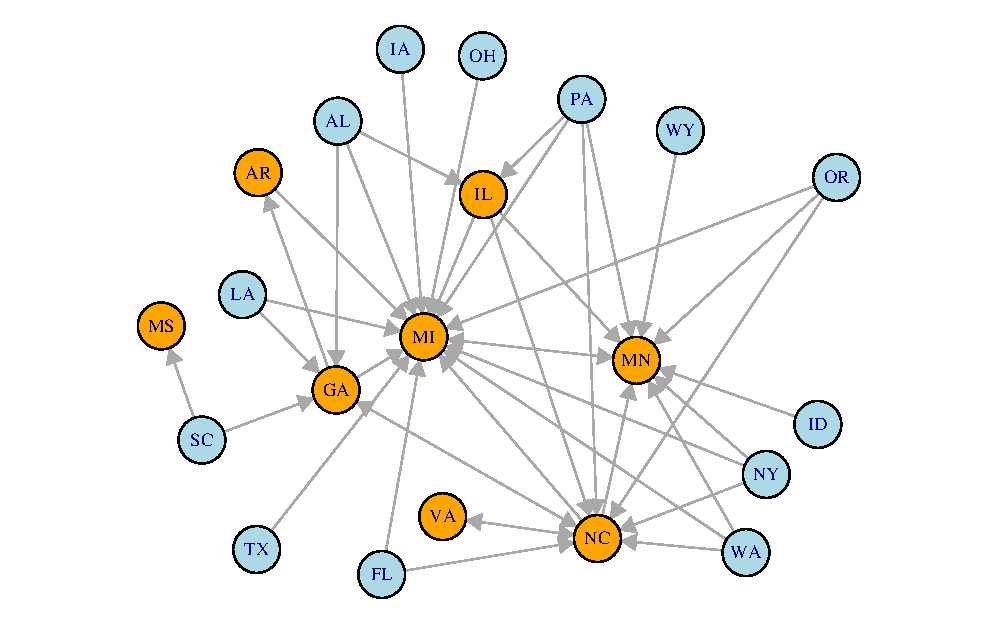
\includegraphics[width=0.6\textwidth]{figs/network.eps}
\end{frame}

\begin{frame}{R的优点}
    \begin{itemize}
        \item \textbf{自由软件}:免费、开放源代码,支持各个主要计算机系统;
        \begin{figure}[htbp]
            \centering
            \includegraphics[width=\linewidth]{figs/downloadr.PNG}
        \end{figure}
    \end{itemize}
\end{frame}

\begin{frame}{R的优点}
    \begin{itemize}
        \item \textbf{强大的图形功能}:强调交互式数据分析,支持复杂算法描述;
        \begin{figure}[htbp]
            \centering
            \includegraphics[width=0.6\linewidth]{figs/plot.jpg}
        \end{figure}
    \end{itemize}
\end{frame}

\begin{frame}{R的优点}
    \begin{itemize}
        \item \textbf{丰富的统计方法}:实现了经典和现代的统计方法,包括:
        \begin{itemize}
            \item 参数和非参数假设检验
            \item 线性回归与广义线性回归等
        \end{itemize}
        \begin{figure}[htbp]
            \centering
            \includegraphics[width=\linewidth]{figs/rc.png}
        \end{figure}
    \end{itemize}
\end{frame}


\begin{frame}{R的优点}
    \begin{itemize}        
        \item \textbf{广泛的使用和扩展包}:统计科研工作者广泛使用R进行计算和发表算法。截止2023年4月,R扩展包的主要分发网站CRAN上已有近19,000个扩展包。
        \begin{figure}[htbp]
            \centering
            \includegraphics[width=\linewidth]{figs/glmtrans.PNG}
        \end{figure}
    \end{itemize}
\end{frame}

\begin{frame}{R的优点}
    \begin{itemize}
        \item \textbf{便捷的程序交互}:R语言提供了友好的交互式环境。
        \item \textbf{多种数据源支持}:可以从多种数据源导入数据,包括文本文件、数据库等。
        \item \textbf{丰富的社区文化}:活跃的社区支持,如GitHub、CSDN。
        
        \begin{figure}[htbp]
            \centering
            \includegraphics[width=0.6\linewidth]{figs/cc.png}
            \caption{R语言支持的数据源}
        \end{figure}
    \end{itemize}
\end{frame}

\begin{frame}{R的下载与安装}
    \textbf{步骤1:} 访问 \href{https://www.r-project.org/}{R项目官网},点击“Download R”。
    \begin{figure}[htbp]
        \centering
        \includegraphics[width=1\linewidth]{figs/s1.png}
    \end{figure} 
\end{frame}
\begin{frame}{R的下载与安装}
    \textbf{步骤2:} 在弹出的镜像(Mirrors)页面上选择合适的镜像入口。如果你在中国,可以直接选择“China”下离你最近的一个镜像。

    \begin{figure}[htbp]
        \centering
        \includegraphics[width=1\linewidth]{figs/s2.png}
    \end{figure} 
\end{frame}
\begin{frame}{R的下载与安装}
    \textbf{步骤3:} 点击对应的操作系统以进行下载。

    \begin{figure}[htbp]
        \centering
        \includegraphics[width=1\linewidth]{figs/s3.png}
    \end{figure} 
\end{frame}

\begin{frame}{R的下载与安装}
    \textbf{步骤4:} 选择 \textbf{base}(基本功能版本),点击 “Install R for the first time”。

    \begin{figure}[htbp]
        \centering
        \includegraphics[width=1\linewidth]{figs/s4.png}
    \end{figure} 
\end{frame}

\begin{frame}{R的下载与安装}
    \textbf{步骤5:} 下载 \textbf{R-x.x.x} 并进行安装。

    \begin{figure}[htbp]
        \centering
        \includegraphics[width=1\linewidth]{figs/s5.png} % 确保使用正确的文件名
    \end{figure} 
\end{frame}

\begin{frame}{RStudio}
    \textbf{RStudio}  是一个功能更强大的R图形界面。安装好R的官方版本后,安装RStudio可以更方便地使用R (\href{https://posit.co/downloads/}{https://posit.co/downloads/})。

    \begin{figure}[htbp]
        \centering
        \includegraphics[width=0.7\linewidth]{figs/rstudio.png}
    \end{figure} 
\end{frame}

\begin{frame}{RStudio的使用}
    \textbf{RStudio界面的主要窗格:}
    \begin{itemize}
        \item 编辑窗格:编写和编辑代码。
        \item 控制台(Console):直接执行R命令。
        \item 环境(Environment):显示当前变量和数据。
        \item 文件(Files):查看项目文件和数据。
        \item 图像(Plots):查看绘制的图像。
    \end{itemize}
     \textbf{如何使用帮助文档:}
    \begin{itemize}
        \item 在控制台中使用 \texttt{?function\_name} 获取帮助。
        \item 访问 \href{https://www.rdocumentation.org/}{RDocumentation}。
    \end{itemize}
\end{frame}
\begin{frame}[fragile]{RStudio的使用:创建文件}
    \textbf{创建R脚本文件的步骤:}
    \begin{enumerate}
        \item 打开RStudio。
        \item 点击 \texttt{File} > \texttt{New File} > \texttt{R Script}。
        \item 在编辑窗格中输入代码。
        \item 点击 \texttt{File} > \texttt{Save} 或使用快捷键 \texttt{Ctrl + S},选择保存位置并命名文件(如 \texttt{example.R})。
    \end{enumerate}
\end{frame}

\begin{frame}[fragile]{R代码的运行}
    \textbf{在RStudio中运行R代码的方法:}
    \begin{itemize}
        \item 在编辑窗格中输入代码后,使用 \texttt{Ctrl + Enter} 运行选中的代码行。
        \item 你也可以在控制台中直接输入代码并按下 \texttt{Enter} 键运行。
        \item 如果要运行选中的或者某行代码,可以点击工具栏中的“Run”按钮。
    \end{itemize}
\end{frame}

\begin{frame}[fragile]{四则运算}
\textbf{四则运算示例:}
\begin{lstlisting}[language=R]
# 计算一个简单的表达式
5+(2.3-1.125)*3.2/1.1+1.23E3
## [1] 1238.418
\end{lstlisting}
\begin{itemize}
    \item 输出结果前的井号(\#)表示这是注释,帮助我们理解代码的含义。
    \item 输出的方括号和数字1是提示性标记,方便我们识别结果位置。
    \item 科学记数法(如\texttt{1.23E3})是如此表示:$1.23 \times 10^3$。
    \item 基本运算符:乘法用星号\texttt{*},除法用正斜杠\texttt{/},乘方用符号\texttt{$\wedge$}。
    \item 记得在输入代码时关闭中文输入法,以免出现错误。
\end{itemize}
\end{frame}


\begin{frame}[fragile]{数学函数}
\textbf{常用数学函数:}
\begin{itemize}
    \item \textbf{平方根、指数、对数:}
    \begin{lstlisting}[language=R]
sqrt(6.25)    # 计算平方根
## [1] 2.5
exp(1)        # 计算自然指数
## [1] 2.718282
 # 计算以10为底的对数
log10(10000) 
## [1] 4
\end{lstlisting}
\end{itemize}
\end{frame}


\begin{frame}[fragile]{数学函数}
    \begin{itemize}
    \item \textbf{取整函数:}
    \begin{lstlisting}[language=R]
round(1.1234, 2)  # 四舍五入
## [1] 1.12
floor(1.1234)     # 向下取整
## [1] 1
ceiling(1.1234)   # 向上取整
## [1] 2
\end{lstlisting}
\end{itemize}
\end{frame}

\begin{frame}[fragile]{三角函数}
\textbf{常用三角函数:}

\begin{lstlisting}[language=R]
pi              # 圆周率
## [1] 3.141593
sin(pi/6)      # 正弦
## [1] 0.5
cos(pi/6)      # 余弦
## [1] 0.8660254
tan(pi/6)      # 正切
## [1] 0.5773503
\end{lstlisting}
\end{frame}

\begin{frame}[fragile]{常量}
\textbf{常量定义:} \\
常量是直接写在程序中的值,包括数值、字符串等。

\begin{itemize}
    \item \textbf{数值型常量:} 整型、单精度、双精度
    \begin{itemize}
        \item 示例: 123, 123.45
    \end{itemize}
    
    \item \textbf{字符型常量:} 使用双引号或单引号包围
    \begin{itemize}
        \item 示例: "Li Ming" 或 'Li Ming'
    \end{itemize}
    
    \item \textbf{逻辑型常量:} 只有 \texttt{TRUE} 和 \texttt{FALSE}
\end{itemize}
\end{frame}

\begin{frame}[fragile]{常量}

\begin{itemize}   
    \item \textbf{缺失值:} 用 \texttt{NA} 表示,常见于数据缺失情况。
    \item \texttt{NaN} (Not a Number): 表示未定义或不可表示的数值,如0除以0。
    \item \texttt{Inf}: 表示正无穷或负无穷,通常在除以零时出现。
\end{itemize}
\end{frame}


\begin{frame}[fragile]{变量}
\textbf{变量定义:} \\
变量用于保存输入值或计算结果。在R中,变量可以保存各种数据类型,如标量、向量、矩阵、数据框和函数。

\begin{itemize}
    \item \textbf{变量名规则:}
    \begin{itemize}
        \item 由字母、数字、下划线和句点组成,不能以数字开头。
        \item 变量名区分大小写,如 \texttt{y} 和 \texttt{Y} 是不同的变量。
        \item 示例: \texttt{x}, \texttt{x1}, \texttt{X}, \texttt{cancer.tab}
    \end{itemize}
    
    \item \textbf{赋值:} 使用 \texttt{<-} 或 \texttt{=} 定义变量。
\end{itemize}
\end{frame}

\begin{frame}[fragile]{作业要求}
请在R中执行文件中的代码,并观察结果。将结果截图或粘贴到Word文档中,最后将文档保存为Word或PDF格式提交。
\begin{itemize}
    \item 请确保在执行代码时,能够观察到每个变量的值和计算结果。
    \item 将结果截图或粘贴到Word文档中,并确保代码及其输出是清晰可见的。
    \item 最后,10月10号前提交到微信群里二维码收件箱。
主题:作业1+学号+姓名,附件为word或pdf。\\
\end{itemize}
\end{frame}


\begin{frame}{}
\centering \Huge
  \emph{Thanks!}
\end{frame}

\end{document}
